%!TEX program = lualatex
\documentclass[a4paper,14pt,openany,oneside]{memoir}

\usepackage{microtype}
\usepackage[hmargin = 2cm, vmargin = 2cm]{geometry}
\usepackage{float}

\usepackage[no-math]{fontspec}
\setmainfont{STIXTwoText}[
    Path            = ./fonts/STIX2/   ,
    UprightFont     = *-Regular.otf    ,
    BoldFont        = *-Bold.otf       ,
    ItalicFont      = *-Italic.otf     ,
    BoldItalicFont  = *-BoldItalic.otf
    ]

\usepackage{unicode-math}
\setmathfont{STIXTwoMath.otf}[Path = ./fonts/STIX2/]

\setmonofont{FiraCode}[
    Path        = ./fonts/FiraCode/ ,
    UprightFont = *-Regular.ttf    ,
    BoldFont    = *-Bold.ttf     ,
    ]

\usepackage{indentfirst}
\usepackage{icomma}
\usepackage{tocloft}
\usepackage{enumitem} 
\makeatletter
\AddEnumerateCounter{\asbuk}{\russian@alph}{щ}
\makeatother
\usepackage{amsmath}
\usepackage{graphicx}
\usepackage{listings}
\usepackage[english,russian]{babel}

% Chapter header format
\renewcommand{\afterchapternum}{.\;}
\renewcommand{\chapnamefont}{\centering\bfseries\large\MakeUppercase}
\renewcommand{\chapnumfont}{\centering\bfseries\large}
\renewcommand{\chaptitlefont}{\centering\bfseries\large}
\renewcommand{\printchaptertitle}[1]{\chaptitlefont\MakeUppercase{#1}}

% Section header format
\setsecnumformat{\csname the#1\endcsname.\;}

% Correct display of the new chapter and section formats with babel
\addto\captionsrussian{
    \renewcommand{\secheadstyle}{\centering\bfseries\large}
    \renewcommand{\subsecheadstyle}{\centering\bfseries\large}
    \renewcommand{\contentsname}{\bfseries Содержание}
    }
    
\pagestyle{plain}
\OnehalfSpacing

\begin{document}
    \chapter{Гидрат метана}
\section{Историческая справка}
\par Гидрат метана относится к классу веществ, называемых газовыми гидратами. Структура газовых гидратов представляет кристаллическую решетку, образованную молекулами воды, в полостях которой помещены молекулы газов. Молекулы воды в этом случае принято называть <<хозяевами>>, а молекулы газа-включения --- <<гостями>>. Соединения включения, имеющие подобную структуру, также принято называть клатратами. Таким образом, газовые гидраты в литературе нередко именуются клатратными гидратами. Газовые гидраты являются твердыми растворами и по структуре схожи с обычным водным льдом за тем исключением, что молекулы-гости газа обеспечивают стабильность характерной именно для газовых гидратов кристаллической решетки, составленной из пяти- и шестиугольников, объединенных в множество многогранников, соприкасающихся гранями. Такая конфигурация из молекул воды, лежащих в вершинах упомянутых многогранников распадается в отсутствии молекул-<<гостей>>.
\par Газовые гидраты впервые были открыты в 1811 году британским химиком Дэвидом Гемфри, который обнаружил [1], что водный раствор хлора кристаллизуется более охотно, чем обычная вода и чистый хлор, который не претерпевает никаких изменений при охлаждении до температуры -40$^{\circ}$. В течение 125 лет с момента данного открытия исследователи в основном занимались поиском как можно большего числа соединений, способных образовывать гидраты, а также описанием их состава и физических свойств. Так, в 1823 году Фарадей предположил химический состав гидрата [2]: \ce{Cl * 10H2O}, что было экспериментально подтверждено Розебомом [3] в 1884 г. В 1888 году Виллард[4] получил гидраты метана, этана и пропана, а также выдвинул гипотезу, что гидраты являются кристаллами. В 1902 году Форкран [5] определил равновесные температуры при атмосферном давлении для 15 различных гидратов.

\par В 1934 году Хаммершмидт [6] обнаружил, что природные газы и вода, в небольшом количестве содержащаяся в объеме газопроводов, образуют гидраты, впоследствии закупоривая их. В связи с этим обстоятельством тематика изучения газовых гидратов стала заметно интереснее и с практической точки зрения, были начаты исследования их термодинамических и кинетических свойств. Так, вскоре был введен строгий контроль за содержанием \ce{H2O} в трубопроводах, а в 1930-1950 годах ученые вели поиск различных ингибиторов, подавляющих рост гидратов, таких как соли хлора,метанол и моноэтиленгликоль.

\par Штакельберг и Мюллер[7,8], а также Клауссен [9] в экспериментах по ренгтеновской дифракции идентифицировали кристаллическую структуру различных газовых гидратов и выделили два её типа: \textit{sI} и \textit{sII}. В 1987 г. группой Рипмистра [10] была обнаружена гексагональная структура гидрата \textit{sH}. Данные типы структур являются наиболее распространенными кристаллическими модификациями газовых гидратов. Сообщалось так же о существовании гораздо реже встречающихся фазах, возникающих сверхвысоких давлениях порядка 1 ГПа, например, Дядиным [11].

\par В 1959 году Ван-дер-Ваальс и Плать\'е разработали [12]  феноменологическую статистическую модель для оценки термодинамических свойств газовых гидратов, которая является наиболее популярной и в настоящее время. Данная модель позволяет предсказывать макроскопические характеристики, такие как температура и давление на основе межмолекулярных потенциалов взаимодействия. Достоинством теории Ван-дер-Ваальса-Платье помимо точности предсказаний является возможность расчета свойств гидратов смесей газов, основываясь на характеристиках чистых газов гидратообразователей.


\par В 1965 году были найдены природные залежи гидратов природных газов на мессояхском газовом месторождении, после чего было обнаружено множество других залежей гидратов на дне океана и в зонах вечной мерзлоты. Возникло понимание, что газовые гидраты могут быть потенциальным источником углеводородной энергии в будущем.
    
\par В 1997 году было обнаружено [13], что полости гидратов могут содержать не обязательно одну, а целых две молекулы-гостя, что было продемонстрировано примере sII гидрата, который в своей большей полости содержал 2 молекулы азота.

\section{Кристаллическая структура}

\par Кристаллическая структура клатратных гидратов природных газов в основном представлена в трех наиболее распространенных формах: \textit{sI}, \textit{sII} и \textit{sH}. Перед тем как обсудить конкретное строение указанных структур, необходимо отметить присущие им общие черты.
\par Молекулы воды, связанные водородными связами, образуют так называемые <<полости>> --- пространственные области в форме многранников, грани которых представляют собой четырехугольники, пятиугольники и шестиугольники. Молекулы воды при этом находятся в вершинах указанных многугольников, а водородные связи направлены вдоль их рёбер. Различные полости соединяются друг с другом, разделяя грани между собой. Получившийся <<ажурный>> каркас носит название решетки-<<хозяина>> Молекулы газов-включений располагаются внутри полостей и называются <<гостями>>. Упомянутые многогранники могут содержать различное число многоугольников в зависимости от типа кристаллической решетки. Обознать их принято используя запись типа $n^m$, где $m$ -- количество многоугольников, составленных из $n$ вершин. В этом случае, например, запись $5^{12}6^4$ будет соответстовать многограннику, построенному из 12 пятиугольников и 4 шестиугольников.
\par Кристаллическая структура \textit{sI} представлена полостями $5^{12}$ и $5^{12}6^2$, структура \textit{sII} полостями $5^12$ и $5^{12}6^4$, а \textit{sH} -- полостями $5^{12}$, $5^{12}6^8$ и $4^35^66^3$. Элементарные ячейки данных кристаллических структур приведены на рис. \ref{fig1.2.1}. На каждую элементарную ячейку приходится соответственно 46, 136 и 34 молекулы воды.

\par Существование нескольких структур объясняется тем фактом, что газовые гидраты образуются молекулами-гостями с различными размерами. Так, \textit{sI}-гидраты образованы молекулами с диаметром от 4,2 до 6 \si{\angstrom}. Примерами являются газы \ce{CH4, C2H6, CO2, H2S}. Молекулы размером меньше 4,2 \si{\angstrom}, такие как водород, азот, криптон, кислород, аргон, а так же молекулы, например, изобутана или пропана диаметром 6-7 \si{\angstrom}, формируют \textit{sII}-гидраты. Наконец, наиболее крупные молекулы размером 7-9 \si{\angstrom}, в совокупности с молекулами меньшего размера, образуют \textit{sH}-гидраты.

\begin{figure}[H]
    \centering
    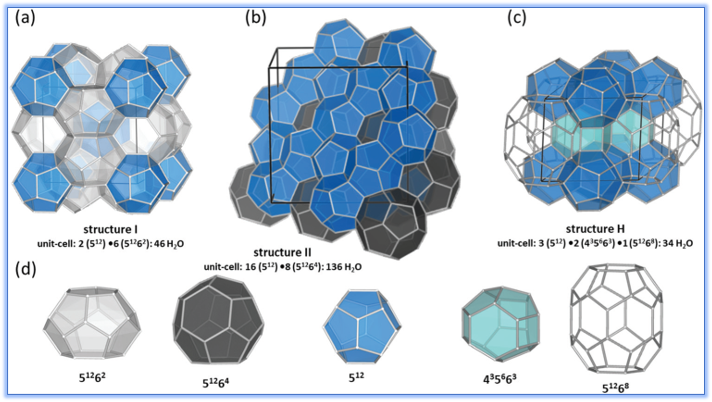
\includegraphics[width=.9\linewidth]{figures/hydrstruct.png}
    \caption{Кристаллическая структура трех наиболее распространенных типов гидратов, а также 5 различных полостей, образующих их. Источник изображения: статья [14].}
    \label{fig1.2.1}
\end{figure}

\par Газовые гидраты состоят из воды на 85\% и по этой причине их часто сравнивают с обычным льдом. Однако в отличие от кристаллической решетки льда, характерная для гидратов структура не может существовать в отсутствие молекул-гостей. Кроме того, гидраты отличаются большей механической прочностью по сравнению со льдом[15], обладают меньшей теплопроводностью[16] и большей теплоемкостью[17] по сравнению с гексагональным льдом.

\par Важно отметить, что газовые гидраты являются нестехиометричными соединениями и идеальных кристаллов газовых гидратов не существует, поскольку молекулы воды всегда присутствуют в большем  количестве чем молекулы газов. Поэтому еще одной характеристикой гидратов является число заполнения полостей. Идеальное стехиометрическое отношение для структуры \textit{sI} составляет $1:5^{3/4}$, \textit{sII} и \textit{sH} -- $1:5^{2/3}$ [18].

\pagebreak
\section{Образование гидратов}
\par Процесс формирования гидратов принято разделять на стадию нуклеации и стадию устойчивого роста кристаллической фазы. Образование газовых гидратов из растворенных в воде газов возможно только в условиях низких температур и высоких давлений. В случае неполярных молекул-гостей, например, метана причина этого заключается в том, что \ce{CH4} является гидрофобной молекулой и имеет низкую величину растворимости в воде порядка $10^{-3}-10^{-5}$ мольных долей при обычных условиях. Однако при понижении температуры до отрицательных величин и увеличения давления до десятков МПа, растворимость  \ce{CH4} увеличивается на два порядка.

\par При исследовании клатратных гидратов под нуклеацией обычно подразумевают явление гомогенной нуклеации, которое представляет собой возникновение в исходной фазе чистого, то есть без наличия примесных молекул или атомов, вещества зародыша новой кристаллической или аморфной фазы, который может состоять из десятков или тысяч частиц. В объеме переохлажденной жидкости вследствие флуктуаций периодически образуются и распадаются кластеры (зародыши) из молекул воды, выстраивающихся вокруг растворенного метана.

\par Зародышеообразование является стохастическим явлением: с некоторой вероятностью зародыш может достичь некоторого критического размера $r$, после чего происходит устойчивый рост новой твердой фазы. Существование критического размера можно объяснить если обратить внимание на величину избытка свободной энергии Гиббса $\Delta G$, который равен сумме поверхностной и объемной частей свободных энергий зародыша:

\begin{equation}
\Delta G = \Delta G_{surf} + \Delta G_{vol} = 4\pi r^2 \sigma + \frac{3}{4}\pi r^3 \Delta g_{vol} \, .
\label{eq1.3.1}
\end{equation}

Здесь $\sigma$ -- поверхностное натяжение на границе раздела зародыша новой фазы и раствора, $\Delta g_{vol}$ изменение свободной энергии в пересчете на единицу объема. Как видно из рисунка \ref{fig1.3.1} $\Delta G$ имеет максимум, соответствующий критическому значению радиуса, который равен

\begin{equation}
    r_{crit} = -2\sigma/\Delta g_{vol} \,.
    \label{eq1.3.2}
\end{equation}
Соотношение \ref{eq1.3.2} можно получить, взяв производную \ref{eq1.3.1} по радиусу зародыша и приравняв её нулю. Соответствующий максимум избытка свободной энергии имеет вид
\begin{equation}
    \Delta G_{crit} = 4\pi\sigma r_{crit}^2 / 3 \,.
    \label{eq1.3.3}
\end{equation}

\begin{figure}[H] 
    \centering
    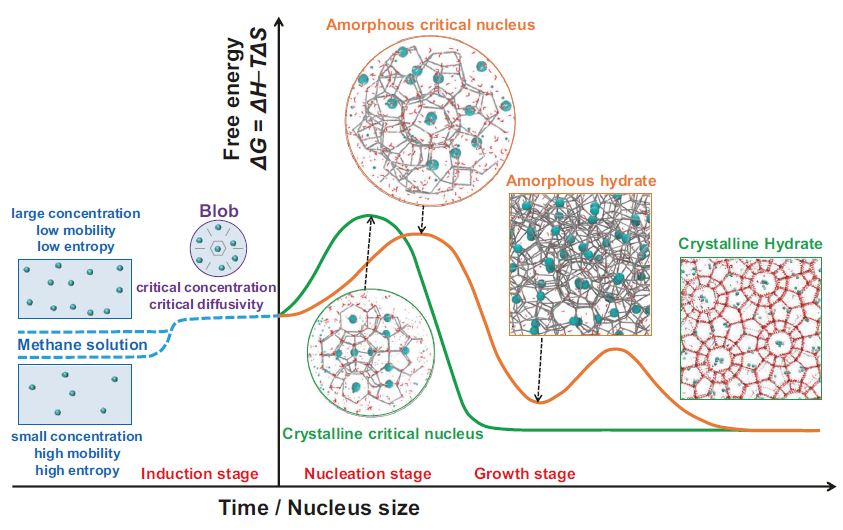
\includegraphics[width=.9\linewidth]{figures/hydrnucl.png}
    \caption{Диаграмма, иллюстрирующая рост гидрата метана [19].}
    \label{fig1.3.1}
\end{figure}

Частота с которой возникают зародыши критического размера в значительной степени зависит от высоты энергетического барьера. При уменьшении величины $r_{crit}$ величина $\Delta G$ так же падает. Критический радиус зародыша может уменьшаться в зависимости от величины пересыщения и переохлаждения $\Delta T$ раствора по зависимости $r_{crit} \propto 1/\Delta T$ [20]. Соответственно увеличивается и вероятность зародышеообразования. 

В настоящее время считается, что образованию зародыша критического размера предшествует возникновение так называемого \textit{сгустка} (с англ. \textit{blob}) -- аморфного кластера[21], состоящего из нескольких молекул газа, разделенных между собой молекулами воды, возникающего вследствие локальных флуктуаций концентрации гостей. Концентрация молекул газов в сгустке выше чем, во всем остальном растворе, с которым он находится в динамическом равновесии. В пределах сгустка периодически возникают и исчезают гидратные полости и их фрагменты, адсорбируя окружающий газ и вновь концентрируя его. Впоследствии может возникнуть кластер критического размера. Критический зародыш может быть как аморфным, так и кристаллическим, в зависимости от того, какие типы полостей образуются первоначально. Соответственно возникает либо аморфная фаза гидрата, которая потом преобразуется в кристаллическую сама по себе со временем или путем отжига, либо же кристалл образуется напрямую.
    \chapter{Молекулярно-динамический подход к изучению гидрата метана}
\section{Метод классической молекулярной динамики}
\par Согласно представлениям классической физики, полностью описать движение произвольной механической системы, состоящей из $N$ частиц можно, если знать координаты $\mathbf{r}_i(t)$ и скорости $\mathbf{\dot{r}}_i(t)$ всех частиц системы $i=1...N$ в любой момент времени $t$. В таком случае движение каждой частицы $i$, находящейся в силовом поле остальных, описывается классическими уравнениями Ньютона:

\begin{equation}
    m_i \mathbf{\ddot{r}}_i(t) = \mathbf{F}_i(t) = \sum\limits_{j=1}^{N} \mathbf{F}_{ij}(t)\,,\quad i = 1\,...\,N \,,
    \label{eq2.1.1}
\end{equation}
где $m_i$ -- масса частицы, $\mathbf{\ddot{r}}_i(t)$ -- её ускорение, $\mathbf{F}_i(t)$ -- результирующая сила, действующая на неё, $\mathbf{F}_{ij}$ -- сила действующая на $i$-ю частицу со стороны $j$-й частицы. Если известна потенциальная энергия парного взаимодействия от расстояния $r_{ij}$ между ними $U(|\mathbf{r}_i-\mathbf{r}_j|) = U(r_{ij})$, то сила выражается следующим образом:

\begin{equation}
    \mathbf{F}_{ij} = -\,\dfrac{\partial U(r_{ij})}{\partial r_{ij}}\cdot\dfrac{\mathbf{r}_{ij}}{r_{ij}}\,.
    \label{eq2.1.2}
\end{equation}
Подставляя \eqref{eq2.1.2} в \eqref{eq2.1.1} получим систему дифференциальных уравнений

\begin{equation}
    \begin{cases}
        \mathbf{\ddot{r}} = -\,\dfrac{1}{m_i}\sum\limits_{j\neq i}^N \dfrac{\partial U(r_{ij})}{\partial r_{ij}}\cdot\dfrac{\mathbf{r}_{ij}}{r_{ij}}\,, \\
        \hfil i = 1\, ...\, N\,.
    \end{cases}
    \label{eq2.1.3}
\end{equation}
Данное векторное уравнение распадается на 3 скалярных. Учитывая, что для полного описания системы нужно решить его для всех $N$ частиц, получаем систему из $3N$ дифференциальных уравнений второго порядка. Также необходимо задать положения частиц и их скорости в начальный момент времени $t_0$:

\begin{equation}
    \begin{cases}
        \mathbf{r}_{i}(t_0) = \mathbf{r}_0\, , \\
        \mathbf{\dot{r}}_{i}(t_0) = \mathbf{\dot{r}}_0\, , \\
        i = 1\,...\,N\,.
        \label{eq2.1.4}
    \end{cases}
\end{equation}

\par Молекулярная физика исходит из представления о том, что любой материал состоит из очень большого числа атомов или молекул, взаимодействующих между собой и находящихся в непрерывном движении. Предполагая, что взаимодействие между ними является классическим, что, как можно показать, справедливо для достаточного широкого класса веществ среди которых встречаются газы, жидкости, кристаллы, аморфные тела, можно применить приведенные выше уравнения для описания поведения этих систем.

\par При этом как известно, состояние макроскопической системы в термодинамически равновесном состоянии определяется сравнительно небольшим набором параметров, такими как температура, давление, плотность, концентрация, химический потенциал, энтропия, внутренняя энергия и другие. В то же время, если учитывать что макроскопические объемы вещества содержат порядка $10^{23}$ атомов или молекул и описываются соответствующим числом степеней свободы, отсюда следует существование огромного числа микросостояний. Поэтому одному макроскопическому термодинамическому состоянию может соответствовать целая совокупность микросостояний, реализующих его, называемая \textit{статистическим ансамблем}. Оперируя методами статистической механики, можно установить связь между макроскопическими и микроскопическими величинами, характеризующими исследуемую систему, к примеру температурой и среднеквадратичной скоростью движения атомов.

\par Аналитическое решение уравнений Ньютона для системы, состоящей из столь большого числа атомов невозможно, однако с развитием вычислительных методов и ростом мощностей ЭВМ появилась возможность численного решения рассматриваемых уравнений и как следствие моделирования поведения физической системы. В этом и заключается сущность метода классической молекулярной динамики: зная начальную конфигурацию системы, потенциальную энергию межмолекулярного взаимодействия (т.н. \textit{потенциал взаимодействия}) и численно интегрируя уравнения Ньютона, можно получить всю необходимую информацию о ней. 

\par Метод молекулярной динамики широко применяется для решения самого широкого круга задач физики, материаловедения, химии и биологии. С помощью него можно исследовать как равновесные, так и неравновесные системы, изучать фазовые переходы, процессы образования дефектов в кристаллах, пор и трещин в материалах, рассчитывать термодинамические и кинетические свойства вещества. Молекулярная динамика применяется для создания лекарственных препаратов и моделирования различных явлений в биомолекулах, например сворачивания белка.

\par Распространенные вычислительные системы на данный момент позволяют рассматривать физические системы размеров порядка десятков нанометров на временных масштабах порядка наносекунд и микросекунд. Такие системы содержат от нескольких тысяч до нескольких десятков тысяч атомов. Хотя эти числа пренебрежимо малы по сравнению с числом атомов в макроскопических системах, все же такого числа частиц достаточно для описания поведения реальных систем.

\section{Скоростной алгоритм Верле интегрирования уравнений движения}

Для интегрирования уравнений \eqref{eq2.1.3} временной интервал $t$, на котором рассматривается эволюция системы, разделяют на множество мелких интервалов шириной $\tau$, называемых временными шагами. В пределах данного промежутка времени движение частиц в системе полагается прямолинейным и равномерным, между ними не действуют силы, поэтому частицы могут перекрыться между собой. Это накладывает ограничение на величину $\tau$, которая должна быть не слишком большой, чтобы не допустить перекрывания. С другой стороны, слишком маленькое значение $\tau$ повлечет за собой увеличение числа временных шагов в пересчете на то же время моделирования $t$, что потребует больших вычислительных ресурсов. Для расчета положения частиц в момент времени $t+\tau$ наиболее часто используется скоростной алгоритм Верле[22]:
\begin{equation}
    \begin{cases}
        \mathbf{r}(t+\tau) &= \mathbf{r}(t) + \mathbf{\dot{r}}(t)\tau+\dfrac{1}{2}\mathbf{\ddot{r}}(t)\tau^2\,, \\
        \mathbf{\dot{r}}(t+\tau/2) &= \mathbf{\dot{r}}(t+\tau/2)+\mathbf{\ddot{r}}(t+\tau)\dfrac{\tau}{2}\,, \\
        \mathbf{\ddot{r}}(t+\tau) &= \dfrac{\mathbf{F}(t)}{m}\,, \\
        \mathbf{\dot{r}}(t+\tau) &= \mathbf{\dot{r}}(t+\tau/2) + \mathbf{\ddot{r}}(t+\tau)\dfrac{\tau}{2}\,.
    \end{cases}
    \label{eq2.2.1}
\end{equation}

\section{Ячейка моделирования. Периодические граничные условия}

Частицы исследуемой системы помещаются в ограниченный объем, имеющий как правило форму параллелепипеда со сторонами $L_x, L_y$ и $L_z$, называющийся \textit{ячейкой моделирования}. Начальные положения частиц в пределах данного объема могут задаваться несколькими способами: случайным образом с использованием генератора случайных чисел или в форме некоторой кристалической решетки, например, ГЦК-решетки. Скорости и направления частиц задаются случайным образом, но так чтобы полученная конфигурация соответствовала некоторой заданной температуре.

\par Для того, чтобы рассматриваемую ячейку моделирования можно было считать частью большой системы, используют периодические граничные условия. Частица, которая покидает ячейку моделирования с некоторой скоростью с одной грани параллелепипеда, не навсегда исчезает из нее, а возвращается с противоположной грани системы с той же скоростью в виде <<образа>>. Это достигается путем создания реплик исходной ячейки моделирования по всем направлениям. То есть получается множество ячеек, частицы в которых движутся точно так же как и в исходной системе.

Любая из координат частицы, например $x_i(t)$, в случае если выполняется условие $x_i(t)\geq L_x$ на следующем временном шаге преобразуется таким образом:
\begin{equation}
    x_i(t+\tau) = x_i(t)-L_x\,.
    \label{eq2.3.1}
\end{equation} 
Если же $x_i(t)\leq 0$, то получим
\begin{equation}
    x_i(t+\tau) = x_i(t)+L_x\,.
\end{equation}
Похожим образом преобразуются проекции расстояни между частицами на координатные оси.

\section{Статистические ансамбли. Термостаты и баростаты}
Молекулярное моделирование может осуществляться с использованием различных статистических ансамблей. Так, в случае если рассматриваемая система является изолированной, реализуется \textit{микроканонический} или $NVE$-ансамбль. Аббревиатура $NVE$ означает что число молекул $N$, объем $V$ и полная энергия $E$ в системе сохраняются.

\par \textit{Канонический} или $NVT$-ансамбль соответствует условиям, когда сохраняются число частиц, объем и температура $T$ в системе. Система находится в тепловом равновесии с термостатом и может обмениваться с ним тепловой энергией.

\par В \textit{изобарически-изотермическом} или $NPT$-ансамбле остаются постоянными число частиц, температура и давление $P$. Для сохранения величины давления используется баростат. Данный ансамбль моделирует условия наиболее приближенные к реальным.

При термостатировании и баростатировании необходимо на каждом временном шаге рассчитывать мгновенные значения температуры и давления в системе.
Как известно, мгновенная температура системы точечных частиц определяется по следующей формуле
\begin{equation}
    T = \dfrac{2}{3Nk_B}\sum\limits_{i=1}^{N}m_{i}\dot{r}_{i}^2\,,
    \label{eq2.4.1}
\end{equation}
где $k_B$ -- постоянная Больцмана.
Давление определяется через вириальное уравнение
\begin{equation}
    P = \dfrac{1}{3V}\sum\limits_{i=1}^N\left(\dfrac{p_i^2(t)}{m} +\sum\limits_{j\neq i}^{N}\mathbf{F}_{i}(t)\cdot\mathbf{r}_{ij}\right)\,,
    \label{eq2.4.2}
\end{equation}
где $p_i(t)=m_{i}v_i(t)$ -- импульс частицы.

Самый простой метод термостатирования называется \textit{методом масштабирования скоростей} и заключается в умножении скоростей частиц $v_i(t)$ в каждый момент времени на коэффициент $\lambda = \sqrt{T_0/T(t)}$, где $T_0$ -- температура термостата. Такой подход, однако, порождает нереалистичную динамику системы.

Существуют более продвинутые алгоритмы позволяющие удерживать необходимые температуры и давления в моделируемой системе, например, термостаты и баростаты Берендсена или Нозе-Гувера.

\section{Радиус обрезания. Список Верле}
Наибольшую часть вычислительных ресурсов при моделировании молекулярной динамики отнимает расчет межчастичных взаимодействий. Так, в пределах одного временного шага, необходимо вычислить $N(N-1)/2$ сил для каждой пары частиц. Такой подход не годится, если рассматриваемое число частиц в системе велико ($N$ порядка 1000 частиц и выше), расчеты будут занимать слишком большое количество времени.
\par Для разрешения данного вопроса стоит обратить внимание на то обстоятельство, что большинство потенциалов межчастичного взаимодействия $U(r_{ij})$ достаточно быстро убывают с увеличением расстояния. Поэтому для них можно считать, что за пределами некоторого расстояния $r_{cut}$ взаимодействие отсутствует, то есть $U(r_{cut}) = 0$ при $r_{ij}\geq r_{cut}$.
\par Получается, что взаимодействие каждой частицы с остальными осуществляется в пределах сферы радиусом $r_{cut}$, где она находится в центре. Л. Верле[23] предложил алгоритм, который при расчете сил, учитывает только данные частицы. Для каждой частицы строится список соседей в пределах упомянутой сферы. Далее сразу за пределами этой сферы строится небольшой сферический слой толщины $\delta r$ толщиной около $0,3\sigma$, где $\sigma$ -- эффективный размер частицы, и определяются частицы находящиеся в этом слое. Список Верле обновляется через некоторое количество временных шагов, в пределах которых частицы из слоя $\delta r$ могут переходить в объем сферы и наоборот.

\section{Модельные потенциалы взаимодействия для описания гидрата метана}
Гидрат метана представляет собой систему, в которой представлены 2 типа молекул: \ce{H_2O} и \ce{CH_4}. Поэтому построение физической модели, позволяющей изучать его свойства методом молекулярной динамики, в сущности сводится к выбору модели межчастичного взаимодействия между молекулами воды, молекулами метана, а так же потенциала их перекрестного межчастичного взаимодействия. Для воды существует множество различных моделей различной степени сложности, такие как, крупнозернистая модель mW[23], трехточечная модель SPC [24], четырехточечная модель TIP4P[25], пятиточечная модель TIP5P[26] и другие. Рассмотрим подробно две модели гидрата метана, использовавшиеся в данной работе. 
\begin{figure}[H]
    \centering
    
\includegraphics[width=.9\linewidth]{figures/watermodels.png}
    \caption{Схематическое изображение строения молекул воды в различных моделях[27]. В трехточечной модели заряды располагаются в положениях точечных масс атомов кислорода и водорода. В четыреточечной модели электрический заряд кислорода смещен относительно массы в позицию M. Аналогичным образом построены пятиточечная и шеститочечная модели.}
    \label{fig2.6.1}
\end{figure}

\section{Модель TIP4P/Ice}
Модель из семейства потенциалов TIP4P[28]. Является широко используемой моделью воды для моделировании гидратов Представляет репараметризацию оригинальной модели TIP4P и хорошо воспроизводит экспериментальную фазовую диаграмму воды, как видно из рис. \ref{fig2.6.2}. TIP4P/Ice также наилучшим образом воспроизводит плотности нескольких кристаллических модификаций льда и температуру плавления льда $I_h$ при атмосферном давления. Модель хорошо воспроизводит температуру плавления $sI$ гидрата метана[https://www.science.org/doi/10.1126/science.1174010].

\begin{figure}[H]
    \centering
    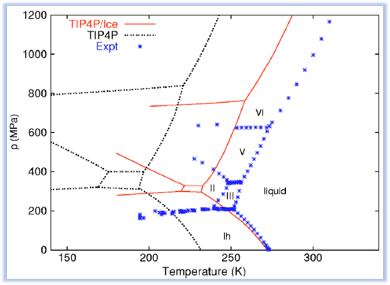
\includegraphics[width=.65\linewidth]{figures/tip4pdiag.png}
    \caption{Сравнение фазовой диаграммы модели TIP4P/Ice с экспериментом и моделью TIP4P[28].}
    \label{fig2.6.2}
\end{figure}

В модели TIP4P/Ice на каждую молекулу воды приходится 3 точечных массы: одна в позиции кислорода, две в позициях водорода (рис. \ref{fig2.6.3}). Позиции зарядов атомов водорода $q_H$ совпадают с позициями их масс, а в случае кислорода заряд $q_O$ смещен относительно положения атома в точку M на расстояние $r_{OM}$ вдоль биссектрисы угла $\angle HOH$. Этот угол жестко зафиксирован, как и расстояния $r_{OH}$ между атомами водорода и кислородом.

\begin{figure}[H]
    \centering
    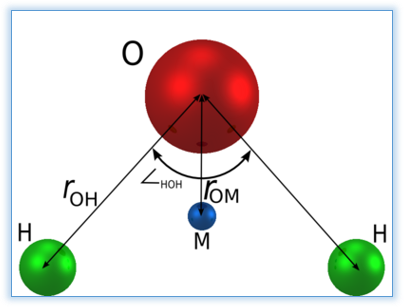
\includegraphics[width=.6\linewidth]{figures/water_mol.png}
    \caption{Молекула воды в модели TIP4P[29].}
    \label{fig2.6.3}
\end{figure}

Потенциал межчастичного взаимодействия представляет собой сумму леннард-джонсовского потенциала и кулоновской энергии взаимодействия точечных зарядов:
\begin{equation}
    \begin{cases}
        E_{LJ} = 4\varepsilon\left[\left(\dfrac{\sigma}{r_{ij}}\right)^{12} - \left(\dfrac{\sigma}{r_{ij}}\right)^6\right]\,,\quad r<r_{cut}\,, \\
        E_{e} = \dfrac{e^2}{4\pi\varepsilon_0}\mathlarger{\mathlarger{\sum}}\limits_{i,j}\dfrac{q_i q_j}{r_{ij}}\,.
    \end{cases}
    \label{eq2.6.1}
\end{equation}
Леннард-джонсовское взаимодействие осуществляется только между атомами кислорода, а электростатическое взаимодействие происходит только между зарядами разных молекул воды. Численные значения параметров модели приведены в таблице ниже:
\begin{table}[H]
    \centering
    \caption{Параметры модели TIP4P/Ice}
    \renewcommand{\arraystretch}{1.8}
    \begin{tabular}{c|c|c|c|c|c|c}
        $\varepsilon_{OO}$ & $\sigma_{OO}$ & $r_{OH}$ & $r_{OM}$ & $\angle$HOH & $q_{O}$ & $q_{H}$ \\ \hline
        0,2109 $\dfrac{\text{ккал}}{\text{моль}}$ & 3,1668 $\si{\angstrom}$ & 0,9572 $\si{\angstrom}$ & 0,1577 $\si{\angstrom}$ & 104.52$^{\circ}$ & −1.1794$e$ & 0.5897$e$ \\ 
    \end{tabular}
    \label{table1}
\end{table}

\section{Модель OPLS-UA}
В качестве модели взаимодействия между молекулами метана вместе с моделью TIP4P часто применяется модель объединенного атома \textbf{\textit{OPLS-United Atom}}[30]. В ней не учитывается внутренняя структура неполярной молекулы \ce{CH4}, метан рассматривается точечная незаряженная частица, межмолекулярное взаимодействие осуществляется через леннард-джонсовский потенциал такого же вида как и в уравнении \eqref{eq2.6.1}. Приведем параметры взаимодействия данной модели:

\begin{table}[H]
    \centering
    \caption{Параметры модели OPLS-UA}
    \renewcommand{\arraystretch}{1.5}
    \begin{tabular}{c|c}
        $\varepsilon_{MM}$ & $\sigma_{MM}$ \\ \hline
        0.294 ккал/моль & 3.73 $\si{\angstrom}$
    \end{tabular}
    \label{table2}
\end{table}

\section{Правила Лоренца-Бертло}
Перекрестное заимодействие между молекулами воды и метана осуществляется также через потенциал Леннард-Джонса, соответствующие параметры $\varepsilon_{OM}$ и $\sigma_{OM}$ рассчитываются по правилам смешивания Лоренца-Бертло[31,32]:
\begin{align}
    \varepsilon_{OM} &= \sqrt{\varepsilon_{OO}\varepsilon_{MM}}\,, \label{eq2.6.2} \\
    \sigma_{OM} &= \dfrac{\sigma_{OO}+\sigma_{MM}}{2}\,.
    \label{eq2.6.3}
\end{align}
Схематично леннард-джонсовское взаимодействие в построенной модели проиллюстрировано на рис \ref{fig2.6.4}.
\begin{figure}[H]
    \centering
    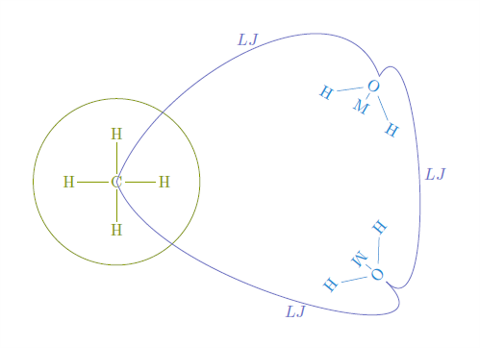
\includegraphics[width=.8\linewidth]{figures/hydrmodel.png}
    \caption{Леннард-джонсовское взаимодействие в модели гидрата метана TIP4P/Ice + OPLS-UA [33]}
    \label{fig2.6.4}
\end{figure}
\pagebreak

\section{Крупнозернистая модель гидрата метана}
В данной модели[34] молекулы воды рассматриваются в рамках модели mW как точечные частицы, взаимодействующие через короткодействующий потенциал Стиллинджера-Вебера[35], состоящий из двухчастичного и трехчастичного вкладов:
\begin{gather}
    E = \sum\limits_{i}\sum\limits_{i<j}\phi_2(r_{ij}) + \sum\limits_{i}\sum\limits_{j\neq i}\sum\limits_{k>j}\phi_3(r_{ij},r_{ik},\theta_{ijk})\,, \label{eq2.13} \\
    %
    \phi_2(r_{ij}) = A\varepsilon\left[B\left(\dfrac{\sigma}{r_{ij}}\right)^4 -1\right]\exp\left(\dfrac{\sigma}{r_{ij}-a\sigma}\right)\,,
    \label{eq2.14} \\
    %
    \phi_3(r_{ij},r_{ik},\theta_{ijk}) = \lambda\varepsilon{[\cos{\theta_{ijk}}-\cos{\theta_0}]}^2\exp{\left(\dfrac{\gamma\sigma}{r_{ij}-a\sigma}\right)}\exp{\left(\dfrac{\gamma\sigma}{r_{ik}-a\sigma}\right)}
    \label{eq2.15}
\end{gather}
$\theta_{ijk}$ определяет угол между частицами $i,j,k$. Постоянные $A, B, \gamma, a, \theta_0$ имеют такие же значения, как и в оригинальной модели для атома кремния, на основе которой получена модель mW. Трехчастичная часть \eqref{eq2.15} потенциала взаимодействия \eqref{eq2.13} построена таким образом, чтобы образование тетраэдрических структур молекулами воды было энергетически выгодно. Значения параметров $\lambda, \sigma, \epsilon$ для воды отличается от таковых для кремния. модель mW воспроизводит экспериментальные значения энтальпии испарения, плотности воды при при температуре 298 К и атмосферном давлении и температуру плавления гексагонального льда. Приведем значения упомянутых модельных параметров в отдельной таблице:

\begin{table}[H]
    \centering
    \caption{Параметры модели mW}
    \renewcommand{\arraystretch}{1.5}
    \begin{tabular}{c|c}
        $A$             & 7,049556277       \\ \hline
        $B$             & 0,6022245584      \\ \hline
        $\gamma$        & 1,2               \\ \hline
        $a$             & 1,8               \\ \hline
        $\theta_0$      & 109,5$^{\circ}$   \\ \hline
        $\lambda_w$       & 23,15             \\ \hline
        $\varepsilon_w$ & 6,189 ккал/моль   \\ \hline
        $\sigma_w$      & 2,3925 $\si{\angstrom}$
        \end{tabular}
    \label{table3}
\end{table}

Молекулы \ce{CH4}, как и в модели OPLS-UA представляются точечными бесструктурными частицами, однако энергия их парного взаимодействия описывается иной формулой \eqref{eq2.13}, где значение $\lambda$ берется равным нулю, то есть трехчастичное взаимодействие отсутствует. Параметры $\sigma_m=4.08 \si{\angstrom}$ и  $\varepsilon_m=0.340$ ккал/моль подобраны таким образом, чтобы эта модель воспроизводила величину энтальпии испарения метана при температуре его кипения $T_m=111.66$ К и давлении $p=1$ атм.

Взаимодействие вода-метан описывается аналогично, вода не образует водородные связи с метаном, поэтому $\lambda=0$. Значения постоянных составляют $\varepsilon_{wm}=0.180$ ккал/моль  и $\sigma_{wm}=4 \si{\angstrom}$. Они выбраны так, чтобы получить наилучшее приближение к экспериментальным значениям температуры плавления \textit{sI} и \textit{sII} гидратов метана, растворимости метана, энтропии и энтальпии диссоциации \textit{sI} гидрата. Модель также дает хорошую оценку величины поверхностного натяжения на границе раздела метан-вода, отличающуюся от экспериментальной на 7\%. 

Недостатками крупнозернистой модели гидрата метана можно отнести переоценку подвижностей метана и воды. Отсутствие вращательных степеней свободы в модели приводит к меньшим на 25\% значениям энтропии и энтальпии диссоциации гидрата. 

Достоинствами являются скорость модели на 2-3 порядка выше скорости атомистических моделей с суммированием по Эвальду, достигающаяся за счет уменьшения числа частиц, короткодействующего потенциала взаимодействия, и возможности использования большого временного шага вплоть до 10 фс.

\section{Идентификация структуры гидратов. Алгоритм CHILL+}
Существуют различные подходы, позволяющие определить в системе наличие фазы гидратов. Например применяются алгоритмы, позволяющие идентифицировать различные полости клатратов $5^{12}, 5^{12}6^2, 5^{12}6^3, 5^{12}6^4$[36] путем нахождения по координатам частиц пятиугольников и шестиугольников, являющихся составными частями полостей гидратов. Еще один подход основан на вычислении параметров ориентационного порядка порядка, зависящих от величины двугранного угла между соседними частицами[37]. В данной работе для идентификации кристаллической и аморфных фаз гидрата метана применяется алгоритм \textit{CHILL+}[38]. В основе алгоритма лежит расчет корреляций параметров ориентацинного порядка[39] молекулы воды с её четырьмя ближайшими соседями. Корреляция $c(i,j)$ локальных параметров ориентационного порядка $l$-й степени  $q_{l}(i)$ рассчитываются по следующей формуле[40]:
\begin{equation}
    c(i,j) = \dfrac{q_l(i)\cdot q_l(j)}{|q_l(i)||q_l(j)|}\,.
    \label{eq2.16}
\end{equation}
Выражение для вычисления $q_{l}(i)$ имеет вид
\begin{equation}
    q_l(i)=\sqrt{\dfrac{4\pi}{2l+1}\sum\limits_{m=-l}^l{|q_{lm}(i)|}^2}\,,
    \label{eq2.17}
\end{equation}
где $q_{lm}(i)$ выражается через сферические гармоники $Y_{lm}(\mathbf{r}_{ij})$:
\begin{equation}
    q_{lm}(i) = \dfrac{1}{4}\sum\limits_{j=1}^4{Y_{lm}(\mathbf{r}_{ij})}\,.
    \label{eq2.18}
\end{equation}
CHILL+ может идентифицировать структуру кубического льда $I_c$, гексагонального льда $I_h$ и гидратов. Авторы алгоритма отмечают то обстоятельство, что в этих трех структурах геометрия водородных связей различается. Выделяют два типа: шахматную (с англ. \textit{staggered conformation}) и заслонённую (с англ. \textit{eclipsed conformation}). На рис. \ref{fig2.11} приведено их графическое представление, а на рис. \ref{fig2.12} они изображены в $sI$-гидрате и льде $I_h$.

\begin{figure}[H]
    \centering
    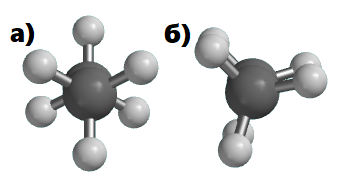
\includegraphics{figures/bonds.png}
    \caption{Шахматная конформация (а) и заслоненная конформация (б)}
    \label{fig2.11}
\end{figure}
\begin{figure}[H]
    \centering
    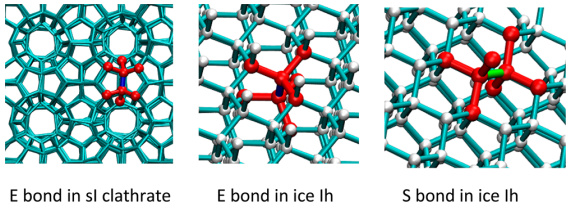
\includegraphics{figures/chillplus.png}
    \caption{Заслоненная конформация и соответствующая заслонённая связь (\textit{E bond}), выделенная синим цветом в $sI$-гидрате и льде $I_h$, шахматная конформация и шахматная связь (\textit{S bond}), выделенная зеленым цветом, в льде $I_h$.}
    \label{fig2.12}
\end{figure}

Вода в составе гидрата образует 4 заслонённые связи, в фазе $I_h$ она имеет 1 заслонённую и 3 шахматные связи, в кубическом льде существуют 4 шахматные связи. Таким образом, по числу связей того или иного вида, можно определить соответствующую структуру. CHILL+ рассчитывает корреляции параметра $q_3$ для каждого ближайшего соседа выбранной молекулы воды, которые для заслоненной конформации принимают значения в диапазоне $-0,05\geq c(i,j) \geq -0,2$, а для шахматной -- $c(i,j)\leq -0,8$.
\end{document}